% !TEX root = paper.tex
\section{Introduction}\label{sec:intro}
\begin{figure}[H]
    \centering
    \begin{subfigure}[t]{0.49\linewidth}
        \centering
        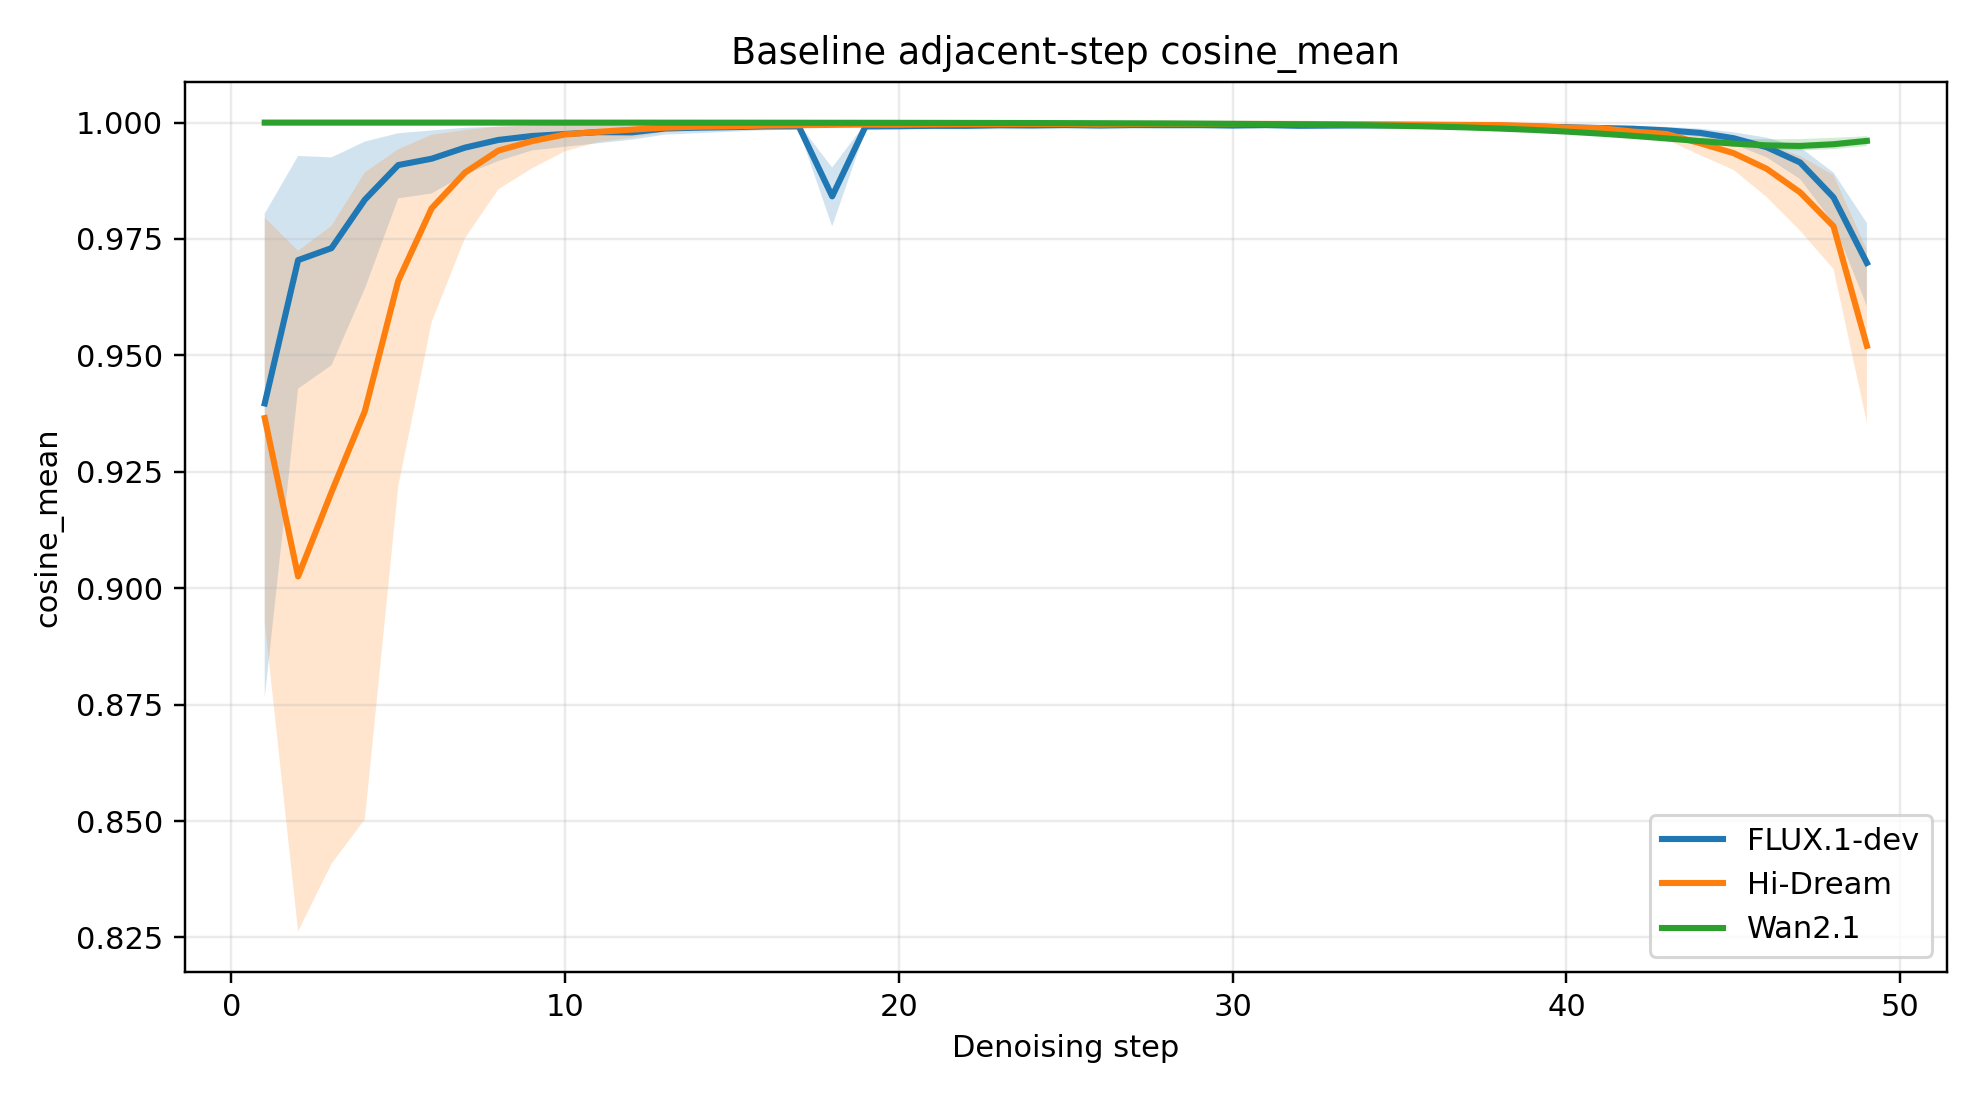
\includegraphics[width=\linewidth]{figures/motivation/cosine_vs_step.png}
    \end{subfigure}\hfill
    \begin{subfigure}[t]{0.49\linewidth}
        \centering
        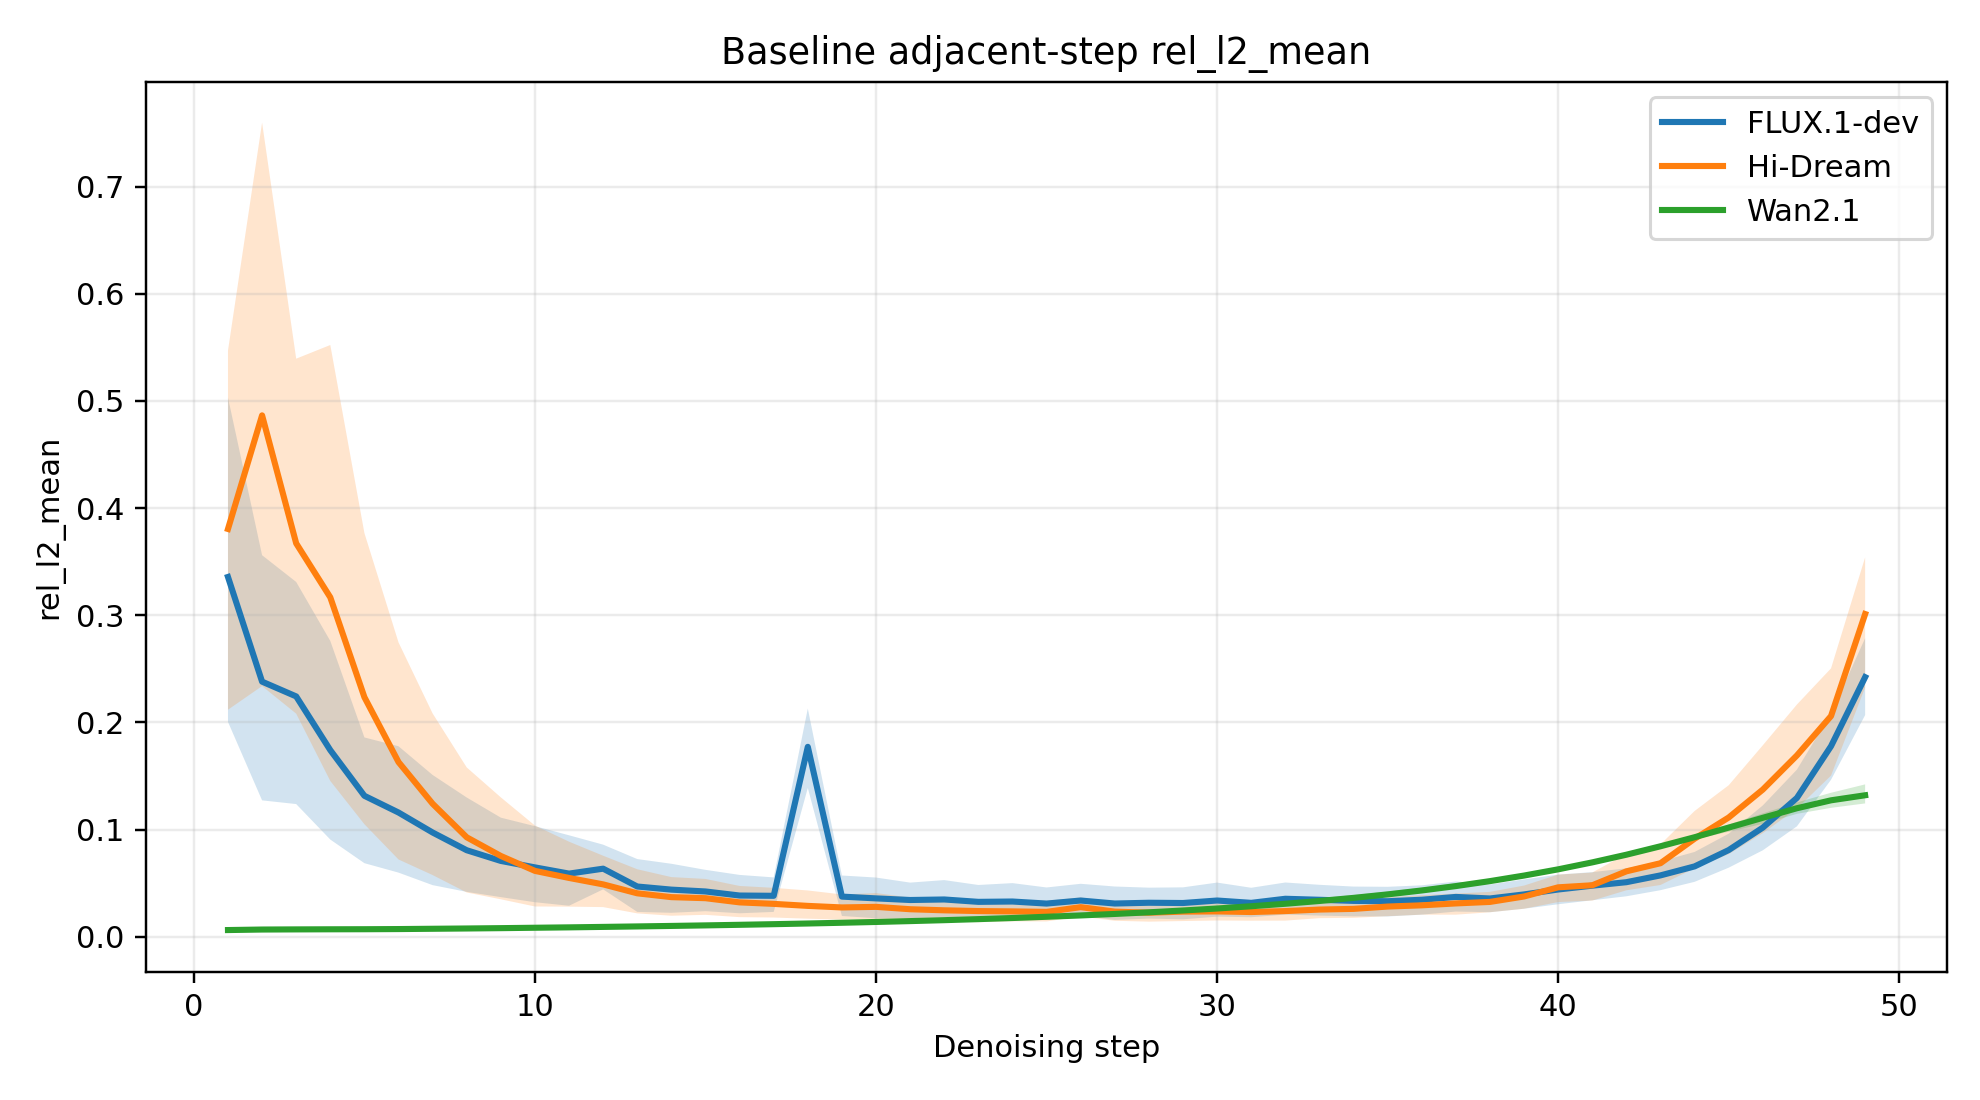
\includegraphics[width=\linewidth]{figures/motivation/rel_l2_vs_step.png}
    \end{subfigure}
    \caption{
        Step-to-step consistency of transformer outputs along the denoising trajectory.
        Left: cosine similarity between transformer outputs at consecutive denoising steps.
        Right: relative $\ell_2$ change between transformer outputs at consecutive denoising steps.
        Curves correspond to FLUX.1-dev, Hi-Dream, and Wan2.1; shaded regions denote the inter-quantile range (p10--p90) over prompts from the DrawBench200 dataset at each step.
    }\label{fig:motivation-latent-similarity}
    \vspace{-15pt}
\end{figure}

Diffusion models \cite{ho2020denoising,
song2020denoising,
dhariwal2021diffusionmodelsbeatgans,
pmlr-v37-sohl-dickstein15,
song2019generative,
rombach2021highresolution}
have emerged as a prominent paradigm in generative modeling,
demonstrating strong empirical performance across a wide range of tasks,
particularly in image \cite{saharia2022photorealistic,chen2023pixartalpha,podell2023sdxlimprovinglatentdiffusion}
and video \cite{videoworldsimulators2024,ma2025latte} synthesis.
To further improve model capacity and generation quality,
recent work has increasingly transitioned
from convolutional U-Net backbones \cite{ronneberger2015unetconvolutionalnetworksbiomedical,ho2020denoising}
to Diffusion Transformers (DiT) \cite{Peebles2022DiT,bao2022all},
which provide a more scalable architecture for high-capacity diffusion modeling.

\begin{figure}[!t]
    \centering
    % 
\includegraphics[width=0.90\textwidth]{figures/architecture/architecture.pdf}
    \caption{%
    \textbf{$\mathrm{D}^3$-Cache Framework:}
    The framework operates through a dynamic adaptive caching mechanism
that leverages DMD-based prediction to determine
which timesteps require full computation
versus feature cache reuse.
At timestep $t_k$, the DMD predictor generates $\hat{\mathbf{y}}_{k+1} = \mathbf{A} \mathbf{y}_k$
based on a linear operator $\mathbf{A}$.
The preview error compares the prediction with the subsequent exact output,
and full computation is triggered when the reuse condition is not satisfied
or the number of reused steps $s_k$ exceeds $S_{\max}$;
otherwise, the predicted transformer output is reused.
A sliding window history enables periodic refinement of the operator and threshold,
allowing adaptation to evolving activation dynamics.
    }
    \label{fig:architecture}
    \vspace{-10pt}
\end{figure}


However, these architectural advances come at a significant computational cost,
resulting in substantially increased inference latency.
This inefficiency is further amplified by the inherently sequential,
multi-step sampling process of diffusion models \cite{shih2023paradigms},
in which each denoising step requires a full forward pass through the network.
% Additionally,
% conventional acceleration paradigms
% such as post-training quantization
% \cite{chen2024QDiT,wu2024ptq4dit,he2023ptqdaccurateposttrainingquantization}
% and knowledge distillation \cite{
%     salimans2022progressivedistillationfastsampling,
%     meng2023distillationguideddiffusionmodels}
% suffer from fundamental limitations:
% both methodologies entail supplementary training procedures,
% which substantially undermines their generalizability
% and practical scalability across heterogeneous model architectures.

Based on the observation that consecutive diffusion steps
exhibit feature similarities,
feature reuse methods \cite{
    Xu_2018,
    wimbauer2024cachecanacceleratingdiffusion,
    selvaraju2024forafastforwardcachingdiffusion,
    zou2024accelerating,
    zou2025rethinkingtokenwisefeaturecaching}
have been proposed to accelerate generation
by strategically caching
and reusing intermediate outputs
across successive denoising iterations.

Existing cache-based methods
typically couple cache reuse with per-model calibration artifacts,
including fitted coefficient tables,
step-dependent reference schedules,
or fixed-order functional expansions.
While effective,
these mechanisms are specified in advance
rather than estimated online from the current feature trajectory.
In practice,
the amount of inter-step change
varies across the denoising trajectory:
aggressive reuse can accumulate drift and erase fine details,
while conservative policies
leave substantial redundancy unexploited.
This motivates a predictive, confidence-aware mechanism
that can adapt reuse decisions online,
skipping computation when dynamics are stable
and falling back when they are not.

To characterize the evolution of transformer outputs along the denoising trajectory,
we quantify the cosine similarity and relative change
between transformer outputs at consecutive steps:
\begin{equation}
    \begin{aligned}
        s_k &=
        \frac{\langle \mathbf{y}_{k-1}, \mathbf{y}_k \rangle}
        {\|\mathbf{y}_{k-1}\|_2 \|\mathbf{y}_k\|_2}, \\
        \delta_k &=
        \frac{\|\mathbf{y}_k - \mathbf{y}_{k-1}\|_2}
        {\|\mathbf{y}_{k-1}\|_2}.
    \end{aligned}
    \label{eq:intro:step-similarity}
\end{equation}
As shown in \Cref{fig:motivation-latent-similarity},
most intermediate denoising steps exhibit cosine similarity close to one
and small relative change, together with narrow inter-quantile bands across prompts,
indicating that adjacent transformer outputs remain strongly consistent
and vary smoothly over these regions of the trajectory.
By contrast,
larger deviations are concentrated primarily in the early and late stages.
These trends suggest that,
over short temporal windows,
the denoising trajectory is strongly coherent
and can be well approximated by a locally linear evolution
in feature space.
These observations suggest the use of a predictive mechanism
capable of capturing local dynamics from short feature trajectories.
Dynamic Mode Decomposition (DMD) \cite{kutz2016dynamic,dey2022dynamicmodedecompositionkoopman}
provides exactly such a mechanism
by fitting a local linear evolution operator to a sequence of snapshots.

This perspective is particularly appealing
relative to existing feature reuse strategies.
TeaCache \cite{liu2024timestep}
and MagCache \cite{ma2025magcache},
for instance,
determine cache reuse through model-specific,
offline-calibrated control profiles,
including fitted rescaling coefficients,
step-wise magnitude-ratio schedules; 
these controls are specified in advance
rather than updated online from the current feature trajectory.
TaylorSeer \cite{TaylorSeer2025}
and HiCache \cite{feng2025hicachetrainingfreeaccelerationdiffusion}
instead extrapolate future features
through Taylor- and Hermite-based analytic expansions,
with the resulting forecasts determined
by the prescribed basis and expansion order.
As the extrapolation order or forecasting horizon increases,
such fixed-form expansions can become more sensitive to approximation error,
leading to noticeable quality degradation under more aggressive reuse.
By comparison,
DMD estimates its evolution operator online from recent output histories,
allowing the extrapolation coefficients to adapt to local dynamics.
Reuse decisions are then made by comparing the predicted and exact next-step outputs,
so that cached outputs are reused only when the observed prediction error
falls below a preset threshold.
This makes DMD better suited to non-uniform timestep spacing,
where prediction difficulty can vary substantially along the denoising trajectory.

% To quantify this phenomenon,
% \Cref{fig:motivation-latent-similarity}
% shows tight inter-quantile bands for most intermediate steps,
% indicating that consecutive timesteps produce highly consistent activations,
% while the first and last few steps exhibit larger variation.
% Inspired by Dynamic Mode Decomposition (DMD) \cite{kutz2016dynamic,dey2022dynamicmodedecompositionkoopman},
% the evolution dynamics
% between consecutive diffusion timesteps
% can be approximated
% by an optimal linear operator
% learned from observed activation sequences.
% The fundamental principle of DMD
% establishes that nonlinear dynamical systems,
% despite their inherent nonlinearity,
% exhibit dynamics
% that can be effectively approximated by linear operators
% in the observation space,
% thereby enabling modal extraction.
% Applying this framework to diffusion models,
% the evolutionary process of diffusion
% can be similarly characterized
% through Dynamic Mode Decomposition.

Motivated by this insight,
we propose $\mathrm{D}^3$-Cache,
a dynamic caching strategy
that leverages Dynamic Mode Decomposition (DMD) to 
predict transformer outputs online
and gate cache reuse with the observed prediction error,
thereby enabling selective skipping of expensive forward passes
without compromising generation fidelity.


\quad In summary,
our contributions are as follows:
\begin{itemize}[leftmargin=*,itemsep=2pt, topsep=0pt, parsep=0pt]
\item \textbf{Empirical Characterization of Inter-Step Dynamics:}
We show that transformer outputs across consecutive diffusion steps
exhibit strong local temporal coherence,
characterized by high cosine similarity and low relative change.
Furthermore, for most intermediate denoising steps,
the output trajectory is well approximated by a locally linear evolution,
providing a concrete basis for dynamical forecasting of cached features.

\item \textbf{$\mathrm{D}^3$-Cache:}
We introduce \textbf{$\mathrm{D}^3$-Cache},
a training-free acceleration framework
that leverages Dynamic Mode Decomposition
to model the short-horizon evolution
of diffusion transformer outputs
from only a small number of recent output snapshots.
Coupled with prediction-error-based gating,
$\mathrm{D}^3$-Cache enables dynamic, online cache reuse
via computationally efficient forecasting.


\item \textbf{Superior Performance of $\mathrm{D}^3$-Cache:}
Comprehensive experiments on state-of-the-art diffusion models
(FLUX.1 \cite{flux2024}, HiDream-I1-full \cite{hidreami1technicalreport}, and Wan2.1 \cite{wan2025})
show that $\mathrm{D}^3$-Cache consistently achieves more than $2.5\times$
computational acceleration.
Under iso-speedup comparisons with existing cache-based acceleration methods,
$\mathrm{D}^3$-Cache delivers substantially better generation fidelity
and superior visual quality across both image and video synthesis tasks.
\end{itemize}
